\chapter{Weryfikacja rozwiązania}

W celu weryfikacji poprawności działania zaiplementowanego systemu zostały
wykonane serie testów. System został przetestowany pod kątem sprawdzenia
podstawowych założeń projektowych tj. poprawności wykrywania anomali, związanych
z natężeniem ruchu, w obsługiwanej sieci oraz możliwości skalowania
aplikacji \textit{sdn\_epc} w celu zwiększenia wydjaności systemu.
Przeprowadzenie testów wymagało przygotowania odpowiednich scenariuszy testowych,
zestawienia dedykowanych topolgi sieciowych oraz stworzenia rozwiązań
pozwalających na zebranie własciwych danych z testowanego systemu. Analiza
tychże wyników pozwoliła na stwierdzenie, czy i w jakim stopniu założenia
projektowe zostały spełnione. Niniejszy rozdział szczegółowo opisuje
poszczególne przypadki testowe oraz prezentuje analizę uzyskanych wyników.

\section{Test działania implementacji algorytmu}

% w jaki sposób sprawdzamy czy algorytm działa? Liczymy entropie, trzeba to
% ująć
 
Poprawność działania implementacji algorytmu służacego do wykrywania ataku
DDoS została sprawdzona w dwóch różnych przypadkach testowych, z których każdy
wykorzystywał nieco inną konfigurację testową topologi sieciowej, jak również
samej aplikacji \textit{sdn\_epc}. Przetestowane zostały przypadki, gdy:
\begin{enumerate}
  \item Ruch wygenerowany w sieci testowej był obsługiwany tylko przez jeden
    węzeł aplikacji \textit{sdn\_epc}.
  \item Ruch wygenerowanych w sieci testowej był obsługiwany przez wiele węzłów
    aplikacji \textit{sdn\_epc} działających w klastrze.
\end{enumerate}
Wykorzystanie takich właśnie przypadków testowych umożliwiło sprawdzenie
poprawności implementacji algorytmu zarówno w przypadku działania systemu jako
pojedynczy węzeł aplikacji \textit{sdn\_epc}, jak również w przypadku, gdy
system działał w klastrze. Drugi przypadek jest znacznie bardziej złożony,
ponieważ rozproszenie procesu obliczania algorytmu na wiele węzłów wprowadza
dodatkowe komplikacje, związane z synchronizacją stanu pomiędzy węzłami w
klastrze.

\subsection{Przypadek testowy z wykorzystaniem jednego węzła aplikacji
  \textit{sdn\_epc}}

Schemat topologii sieciowej, wykorzystanej w przypadku, gdy tylko jeden węzeł
aplikacji jest zaangażowany w przetwarzenie ruchu został przedstawiony na
Rys. \ref{fig:entropia_scheme}.

\begin{figure}[h]
\centering
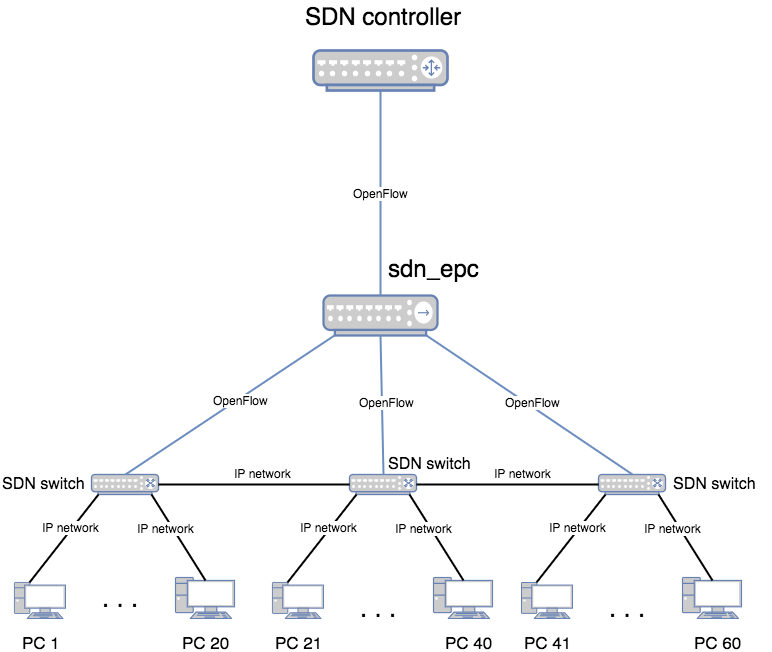
\includegraphics[width=\textwidth]{entropia_scheme}
\caption{Schemat topologii sieciowej z wykorzystaniem jednego węzła aplikacji
  \textit{sdn\_epc}.}
\label{fig:entropia_scheme}
\end{figure}

W topologii przedstawionej na Rys. \ref{fig:entropia_scheme} wszystkie przełączniki
obsługujące ruch pomiędzy węzłami końcowymi (\textit{PC N}) komunikują się z
kontrolerem (\textit{SDN controller}) poprzez jeden węzeł aplikacji
\textit{sdn\_epc}. Wykorzystując taką konfigurację sieci, tylko jeden węzeł
\textit{sdn\_epc} przetwarza wiadomości \mbox{\textit{PACKET\_IN}} protokołu
\textit{OpenFlow}, wymieniane pomiędzy poszczególnymi przełącznikami, a
kontrolerem, w celu obliczenia entropii pakietów przesyłanych w sieci.